\section{Major scale}
\begin{definition}[Tetrachord]
    A 4-note scale segment with the following steps: $W-W-H$.
\end{definition}

\begin{definition}[Major scale]
    A 8-note scale made up of 2 tetrachords, joined by a whole step.
\end{definition}

$$\underbrace{W-W-H}_{T1}-W-\underbrace{W-W-H}_{T2}$$

\begin{figure}[h]
    \begin{center}
        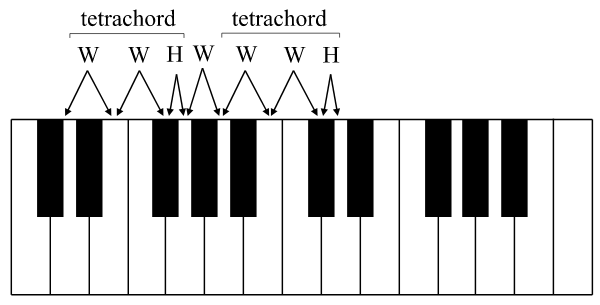
\includegraphics[width=0.6\textwidth]{img/tetrachord}
        \caption{Tetrachords in a (D) major scale}
    \end{center}
\end{figure}

A major scale uses all the 7 notes in order. No one is skipped and there are no duplicates.

\subsection{Key signatures}
There are 15 major key signatures:
\begin{itemize}
    \item 1 with no accidentals: C Major.
    \item 7 with $1$ to $7$ flats.
    \item 7 with $1$ to $7$ sharps.
\end{itemize}

\begin{figure}[h]
    \begin{center}
        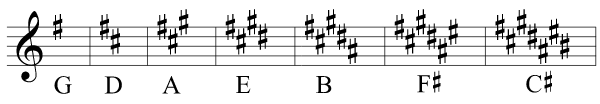
\includegraphics[width=0.8\textwidth]{img/majorsharp}
        \caption{Major key signatures (sharps)}
        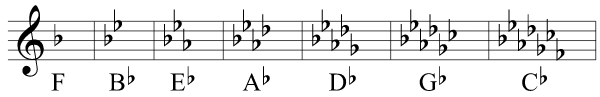
\includegraphics[width=0.8\textwidth]{img/majorflat}
        \caption{Major key signatures (flats)}
    \end{center}
\end{figure}
A key signature can be quickly identified with the following mnemonic:
\begin{itemize}
    \item With \emph{sharps}: +1 half step from the last ``sharped note''.
    \item With \emph{flats}: the second to last flat is the key (along with the flat).
\end{itemize}

\section{Minor scales}
In contrast to major scales, there are 3 different minor scale forms. They all follow the following formulas, while the melodic minor is only used as an \emph{ascending} scale (the \emph{descending} part is the same as the natural minor scale).
\begin{figure}
    \begin{center}
        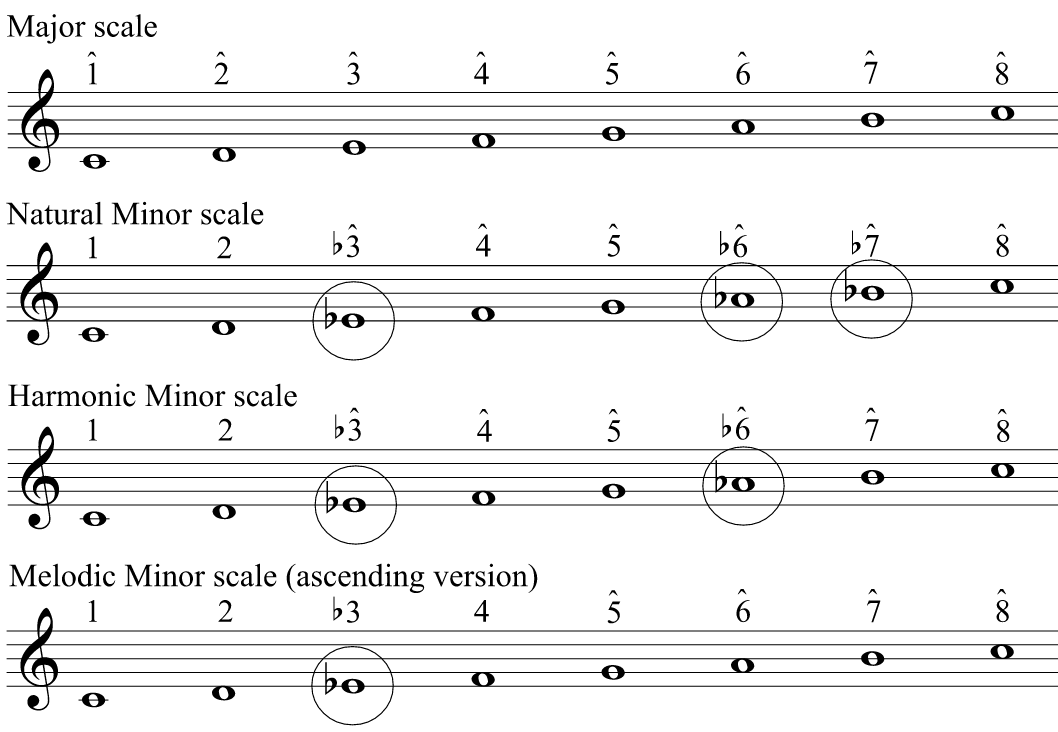
\includegraphics[width=0.8\textwidth]{img/minorscales}
        \caption{Minor scales}
    \end{center}
\end{figure}

\subsection{Harmonic minor scale}
The harmonic minor scale was born as a way to obtain a stronger resolution to the tonic. In fact, the lowered $\hat 7$ scale degree in the natural minor scale leads to a steep resolution to the tonic (a whole step).

So, the harmonic minor scale \emph{raises} the $\hat 7$ scale degree so as to obtain a so-called \textbf{leading tone}. In this way we are able to use a smoother resolution to the tonic from the $\hat 7$ scale degree.

The scale is called \emph{harmonic} minor, because the chords usually come from this harmonic scale (if this is the case, the dominant triad is the same as its major scale counterpart, and they fulfill the same role; the other chords are different between the two modes).

\subsection{Melodic minor scale}
The melodic minor scale shows its purpose in a similar manner as the harmonic minor scale. If we were to use an harmonic minor scale for a resolution then we probably want a passage with ends with $\hat 6 \hat 7 \hat 8$. Note however that in this case we have the same problem as before: the distance between $\hat 6$ and $\hat 7$ is too steep in the harmonic minor scale.

Therefore, we \emph{raise} also the $\hat 6$ scale degree, obtaining the melodic minor scale.

The scale is called \emph{melodic} minor because it shows its purpose during melodic passages which lead to a tonic resolution. In the Common Practice period (1600-1900), minor melodies often followed this scale pattern.

\subsection{Key signatures}
In respect to the major keys, minor keys can be derived by adding 3 flats (or subtracting sharps and adding flats if needed).

In doing so, the corresponding major scale will also have three of its scale degrees lowered, resulting in what is called a \textbf{parallel} minor scale.

\begin{definition}[Parallel scale relationship]
    Two major / minor scales with the same $1^{st}$ scale degree.
\end{definition}

On the other hand, if it is the key signature to be shared, then we call it a \textbf{relative} minor key.

\begin{definition}[Relative key relationship]
    Two major / minor key signatures with the same key signature.
\end{definition}

\section{Circle of fifths}

\begin{figure}
    \begin{center}
        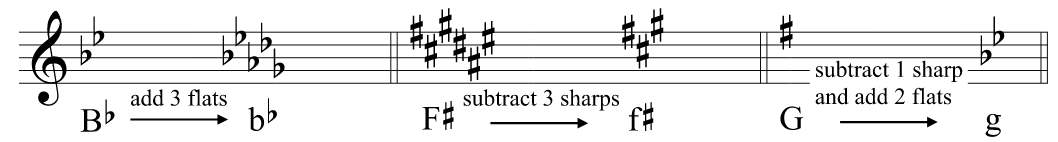
\includegraphics[width=0.8\textwidth]{img/parallel}
        \caption{Parallel relationship}
    \end{center}
\end{figure}

The circle of fifths is a convenient aid for the visualization of both minor and major keys and scales:
\begin{itemize}
    \item To the right, we add sharps / remove flats and we go up a $5^{th}$.
    \item To the left, we remove sharps / add flats and we go down a $5^{th}$.
\end{itemize}
It also provides some interesting insights into the key structure:
\begin{itemize}
    \item Given a note, the next note clockwise is its dominant.
    \item Given two adjacent keys, their scales share $\frac 6 7$ of the notes (e.g. C Major and G Major differ only by the F\#).
    \item In 18th century music often a key modulated itself only to the its 5 other neighboring keys (because they shared $\frac{6}{7}$ notes). These keys and its relative minor are the 6 most \emph{closely related keys}, while others are said to be \emph{distantly related}. In fact, the key on the opposite side of the circle of fifths is said to be the most distantly related.
    
    Beethoven was one of the first composer to deviate from this trend.
\end{itemize}

\begin{figure}
    \begin{center}
        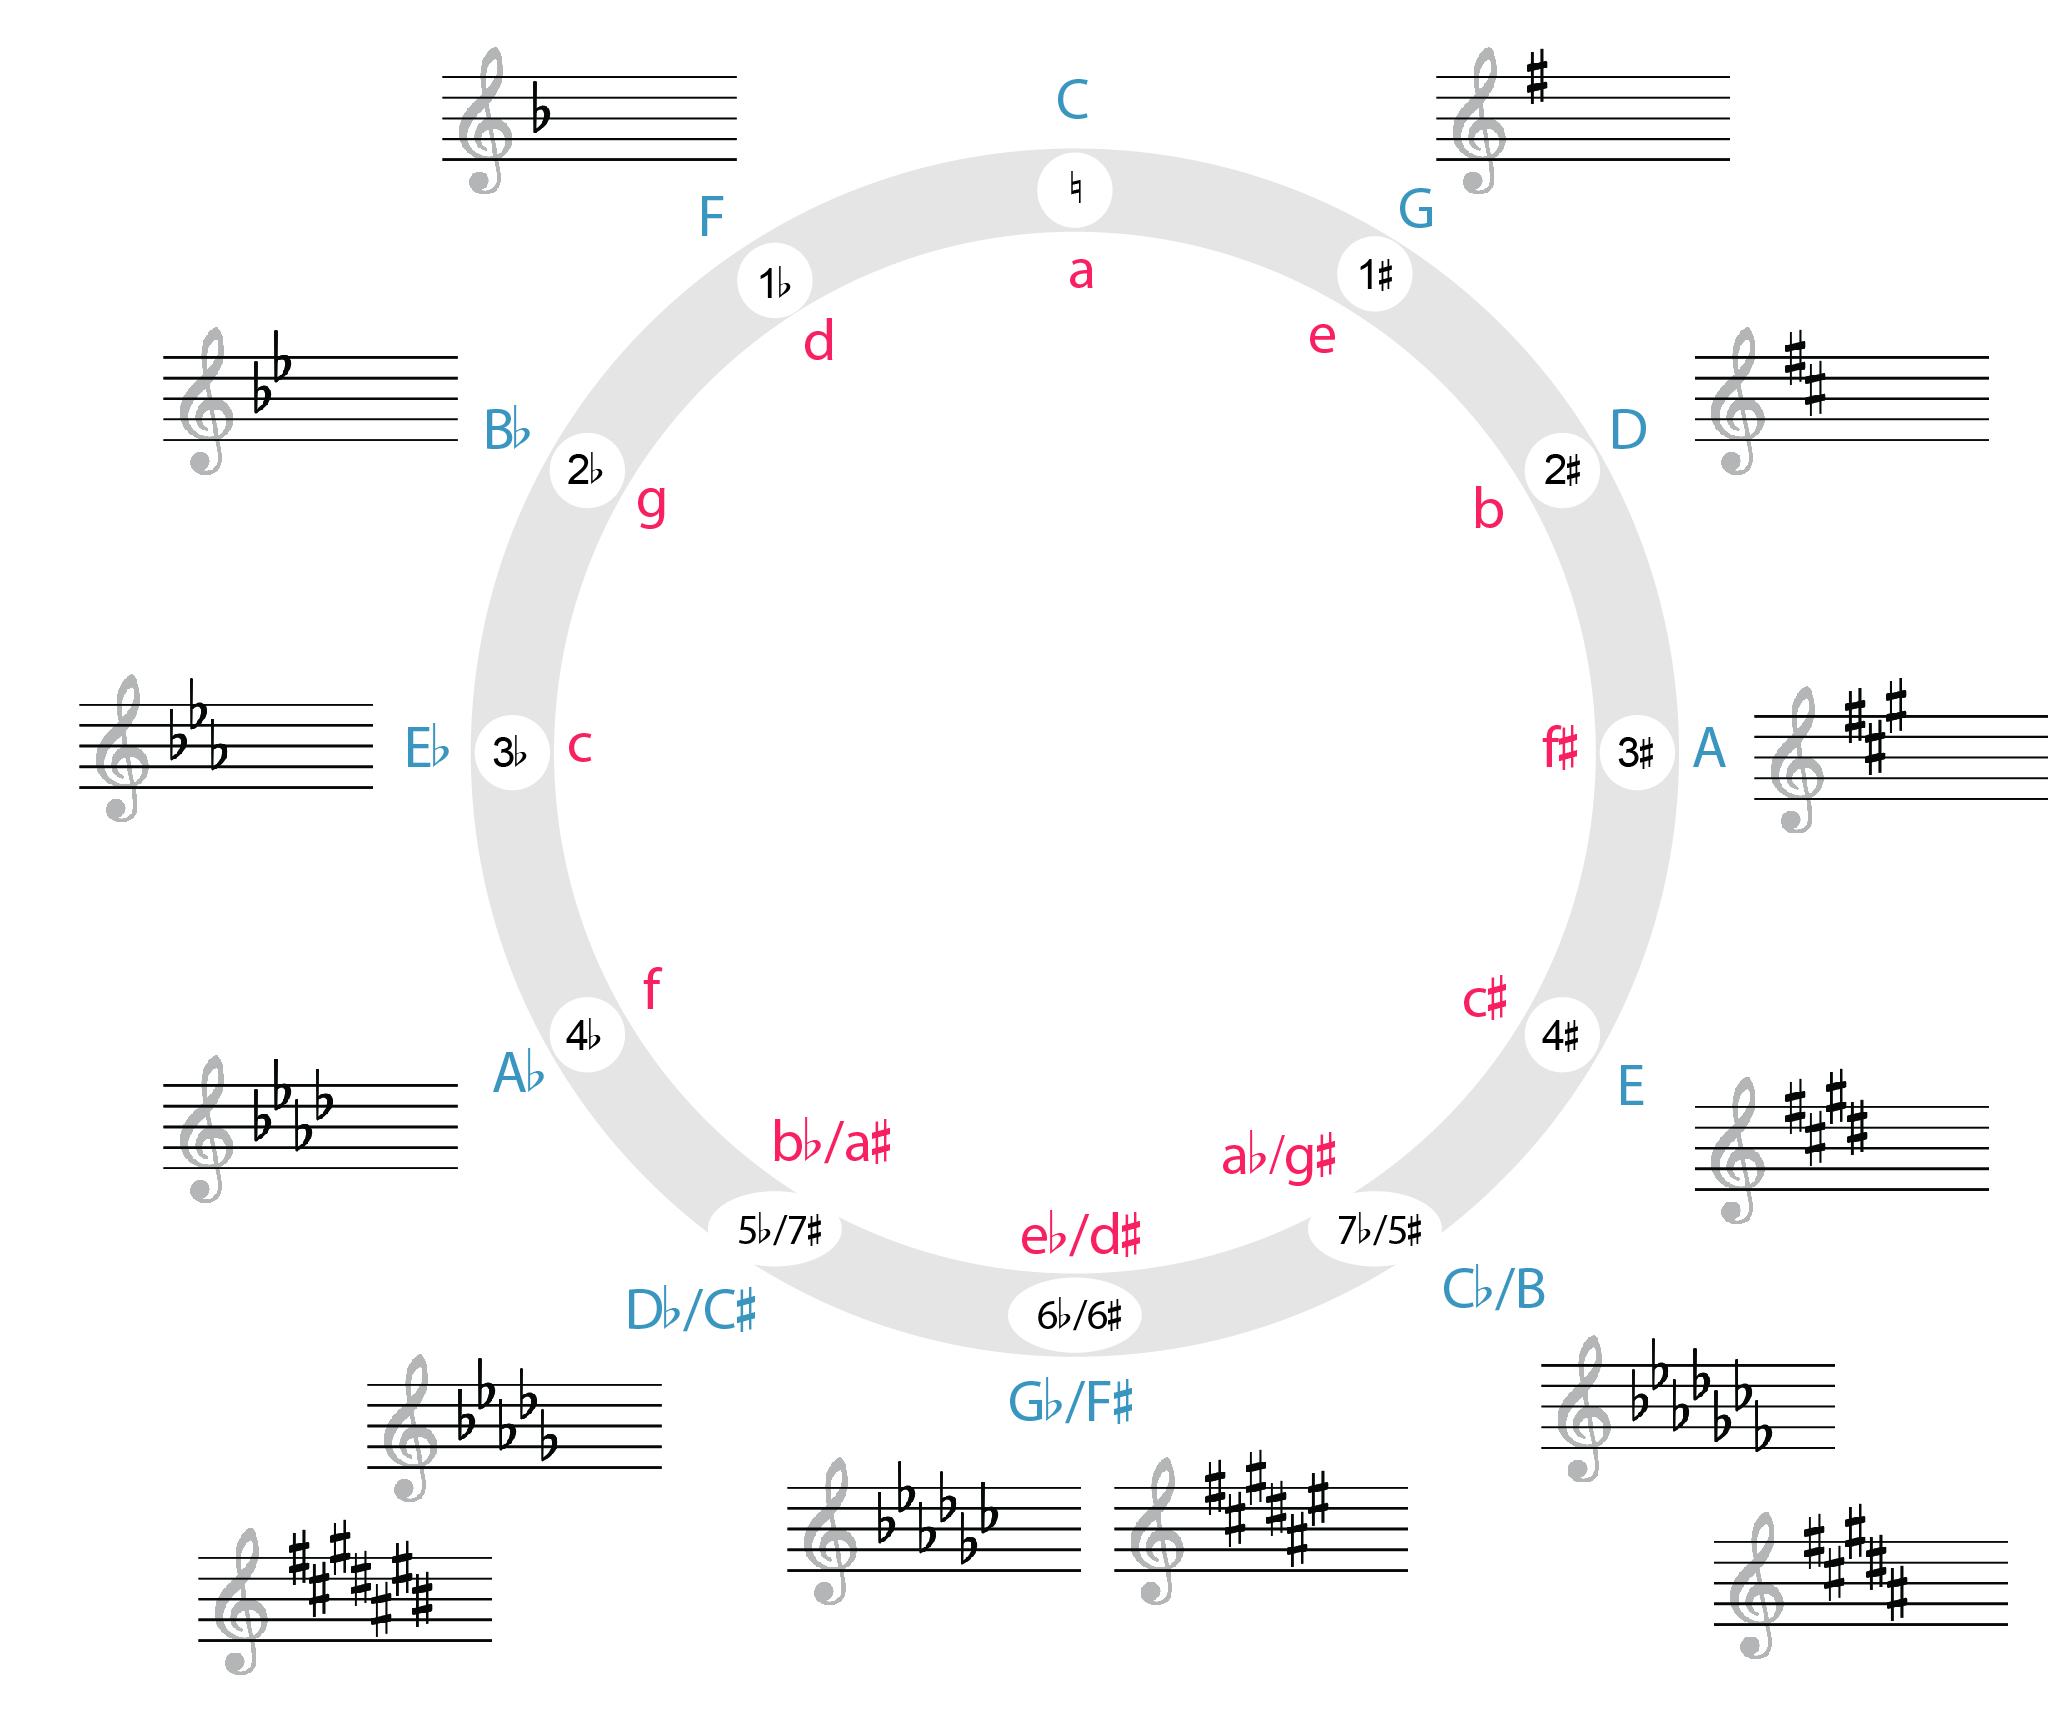
\includegraphics[width=0.8\textwidth]{img/circle}
        \caption{Circle of fifths}
    \end{center}
\end{figure}

\section{Key identification}
\begin{definition}[Key ($\approx$)]
    The \textbf{tonic} and the \textbf{mode} the piece ``is in''.
\end{definition}

What does it mean for a piece to ``be in a key'' (say, the key of C Major)? It means\footnote{Assuming we are talking about \emph{tonal music}.}:
\begin{itemize}
    \item The most important note in the piece (the one that feels like ``home'') is the first scale degree of our scale.
    \item Notes from the key scale (say, the C Major scale) seem like to belong to the piece, while notes from other scales (say, the C minor scale) seem to be extraneous.
\end{itemize}

Given a piece of sheet music we can devise its key as follows:
\begin{enumerate}
    \item Through the number of flats / sharps we restrict ourselves to 2 key signatures: a major one and a minor one.
    \item The tonic can help us do the final discrimination. Usually the tonic note is located at the beginning / end of the piece either in the lower or upper parts (as we want to look for the piece\emph{resolution}, often the tonic can be devised from the last note).
\end{enumerate}

\subsection{Key modulation}
\begin{definition}[Key modulation]
    A temporary change of keys.
\end{definition}

A key modulation can be notated with a text marking like $G:5$, which indicates a modulation to the $G$ as the tonic for the following measures.

A key modulation may or may not be highlighted by a key signature change in the sheet music. When this happens, usually a note or chord is used as a \emph{pivot} for the key modulation; said note or chord is usually in common between the two keys (albeit maybe with different roles).

\begin{definition}[Pivot]
    A common note / chord between two keys, used as for pivoting between the two keys.
\end{definition}

A weaker form of modulation is \textbf{tonicization}, in which a different note is briefly used in place of the actual key's root.

Through leading tones or secondary dominants it is easy to \emph{tonicize} other notes.

\begin{definition}[Tonicization]
    Very briefly treat a different note as the tonic for a piece in a given key.
\end{definition}

\section{Diatonic scale / modes}
\begin{definition}[Diatonic scale]
    A collection of all the seven note pitches in order.
\end{definition}

The diatonic scale can be thought as a \emph{meta-scale}. Its general formula is any shift of the major scale formula, thus we have 7 possible diatonic scale \textbf{modes}.

\begin{definition}[Diatonic mode]
    A specific instance of a diatonic scale.
\end{definition}

In fact, both the major scale and the (natural) minor scale are diatonic modes. The diatonic modes are called through greek names, where {\color{OrangeRed}Ionian} and {\color{RoyalBlue}Aeolian} are the major and (natural) minor scales, respectively.

\begin{center}
    \begin{tabular}{r|c|l}
        \textbf{Mode} & \textbf{Intervals sequence} & \textbf{Example with white keys} \\
        \hline
        {\color{OrangeRed}Ionian} & $W-W-H-W-W-W-H$ & $C-D-E-F-G-A-B$ \\ 
        Dorian & $W-H-W-W-W-H-W$ & $D-E-F-G-A-B-C$ \\
        Phrygian & $W-W-H-W-W-W-H$ & $E-F-G-A-B-C-D$ \\
        Lydian & $W-H-W-W-W-H-W$ & $F-G-A-B-C-D-E$ \\
        Mixolydian & $H-W-W-W-H-W-W$ & $G-A-B-C-D-E-F$ \\
        {\color{RoyalBlue}Aeolian} & $W-W-W-H-W-W-H$ & $A-B-C-D-E-F-G$ \\
        Locrian & $W-W-H-W-W-H-W$ & $B-C-D-E-F-G-A$ \\
    \end{tabular}
\end{center}

\section{Scale degrees and functions}
In a scale there are seven scale degrees, each of them with a different name.

These are the three most important degrees:
\begin{itemize}
    \item $\hat 1$ / \textbf{Tonic}: the center of gravity of a tonal piece of music. Often it ends a piece of music in a given key, which is identified exactly by that tonic.
    \item $\hat 5$ / \textbf{Dominant}: mainly used as a springboard to the tonic.
    \item $\hat 3$  / \textbf{Mediant}: it was used as an helper towards the dominant.
    \item $\hat 2$ \textbf{Supertonic}: can also be used as a \emph{dominant to a dominant}, also called a \textbf{secondary dominant}.
    \item $\hat 7$ / \textbf{Leading tone}: is the most unstable scale degree, which has a strong tendency to resolve to the tonic.
    \item $\hat 4$ / \textbf{Subdominant}: can be both stable or unstable.
    \begin{itemize}
        \item Dominant context $\Rightarrow$ unstable (wants to resolve to $\hat 3$).
        \item Tonic context $\Rightarrow$ stable ($\hat 3$ is its leading tone).
    \end{itemize}
\end{itemize}
Together, these 3 scale degrees form the \textbf{tonic triad}, which is the center of the \emph{harmony} (while the tonic is the center of the \emph{melody}).

\begin{definition}[Tonic triad]
    The triad formed by the $\hat 1, \hat 3, \hat 5$ scale degrees.
\end{definition}

Instead, if we build the triad on the \emph{dominant}, we gather the \textbf{dominant triad}, which strongly wants to resolve to the tonic (triad). The \textbf{mediant triad} instead often sounds pretty stable.

\begin{definition}[Dominant triad]
    The triad built on the $\hat 5$ scale degree.
\end{definition}

\begin{figure}
    \begin{center}
        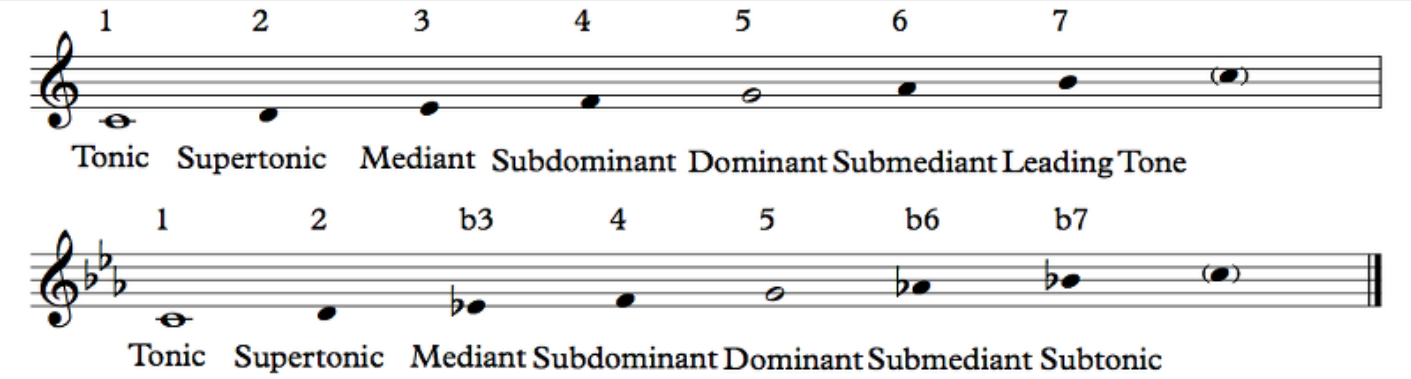
\includegraphics[width=\textwidth]{img/degrees}
        \caption{Scale degree names}
    \end{center}
\end{figure}

\section{Chromaticism}
When we use notes which are outside of our scale we are doing chromatic alterations. This may have two different purposes:
\begin{itemize}
    \item \textbf{Modal mixture}. In modern music theory this is often referred just as \emph{extended tonality}.
    \item Introducing different leading tones (even for scale degrees different than $\hat 7 \to \hat 1$).
    
    Examples: \# 1 resolves to 2, b2 resolves to 1, etc. Notice how the accidental disambiguates between enharmonic notes, building up an expectation to where the note is supposed to resolve\footnote{This does not hold for b3: it is stable.}.
\end{itemize}

\begin{definition}[Modal mixture]
    Using a note from a different mode.
\end{definition}

\begin{definition}[Sublimation]
    When a note resolves to a different note than the one it is intended to resolve to, while mainaining a pleasuring transition.
\end{definition}